\section{State of the art}
In this section we will present a few of the current annotation tools available on the
web, extracting the most relevant features that were taken into account when building
\KAT.

Different types of web-based projects will require different approaches to annotations,
allowing us to distinguish between 2 main categories:
\begin{enumerate}
\item \defemph{Dynamic annotations}: implemented by systems which allow the annotation of
  the text itself. In such a system, the anchor of an annotation is a piece of digitized
  text.
\item \defemph{Static annotations}: implemented by systems which allow the annotation of a
  specific region of content. In this case, the anchor of an annotation is the fixed,
  in-page, position of the annotated region.
\end{enumerate}
Digitized, mathematical text lays in the center of our research direction during this
project and, for this reason, we are going to focus mainly on the first category. However,
in order to have a complete overview of the available features, the last subsection of
this part presents one example from the second category.

An important aspect of our desired system is that, even though it is very close to a
dynamic annotation system, we are looking for a more stable and semantically rich format,
such as \textsf{OMDoc}, to anchor the annotations.

\subsection{the brat Annotation Tool}

brat~\cite{brat:on} Is a web based tool for text annotation. It is designed in particular
for structured annotation, where the notes are not freeform text but have a fixed form
that can be automatically processed and interpreted by a computer and implicitly belongs
to the category of dynamic annotation tools.
\begin{figure}[ht]\centering
 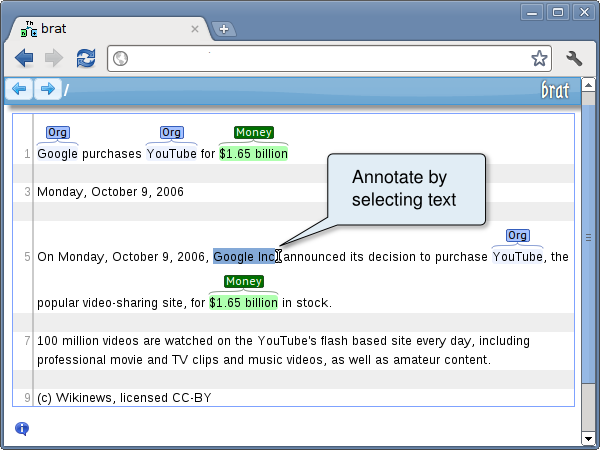
\includegraphics[width=3.7in]{figures/brat}
 \caption{Annotation with brat}\label{fig:brat}
\end{figure}
The most important features that we identified were:
\begin{enumerate}
\item The text must be preprocessed into a particular, fixed format before being
  annotated.
\item There are 2 types of annotation supported:
  \begin{itemize}
  \item text span annotations: simple annotation of a piece of text:
   \begin{center}
     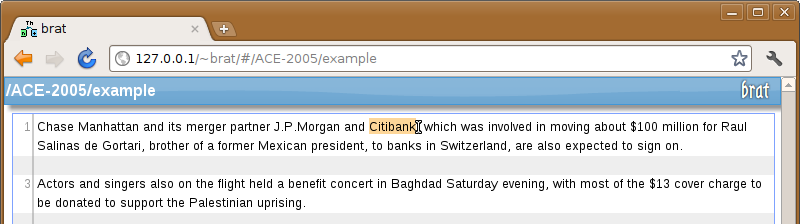
\includegraphics[width=3.5in]{figures/brat-text-span}
   \end{center}
   
  \item relation annotations: two separated pieces of text are annotated and a connection between them is created:
    \begin{center}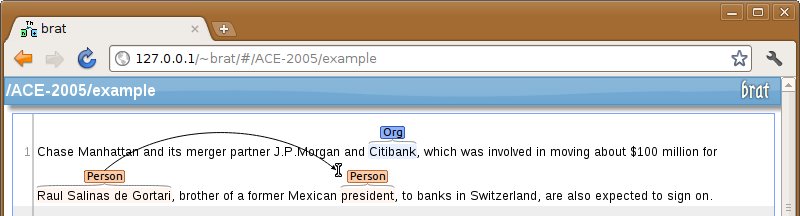
\includegraphics[width=3.5in]{figures/brat-relation}\end{center}
  \end{itemize}
\item Extensive search functionality for annotations, see Figure~\ref{fig:brat-search}
\item Export interface: annotations can be exported in an internal format, which can then
  be converted in other formats such as PDF or HTML. Furthermore, visualizations can be
  exported as well, into SVG and bitmap formats (PNG).
\item Each annotation is accessible by URL: every brat annotation can be uniquely
  addressed within the brat server. Together with the URL of the server, this form of
  addressing provides a globally unique address for every brat annotation.
\item Brat provides a validation system for its annotations: the admin can define
  validation grammar rules, forcing the user to adhere to a specific annotation format.
\item Annotations are anchored based on a word-counter: this makes the annotated text
  unchangeable and constitutes one of our main concerns regarding the system.
\end{enumerate}
\begin{figure}[ht]\centering
  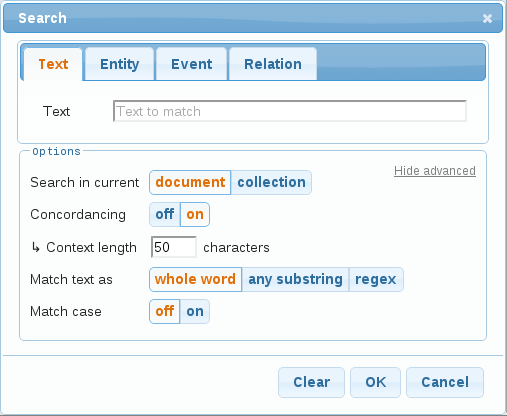
\includegraphics[width=3.5in]{figures/brat-search}
  \caption{Search in brat}\label{fig:brat-search}
\end{figure}

\subsection{Yawas Annotation Tool} 
Yawas~\cite{yawas:on} is an annotation system designed as an extension for Firefox and
Google Chrome; see Figure~\ref{fig:yawas} It is different than the other systems that we
analyzed in that the annotation doesn't belong to the text but to the user. After
installing the extension, the use can navigate to any page and can highlight any piece of
text. The annotation is saved in the user's google account and is displayed every time the
user accesses the page.

\begin{figure}[ht]\centering
  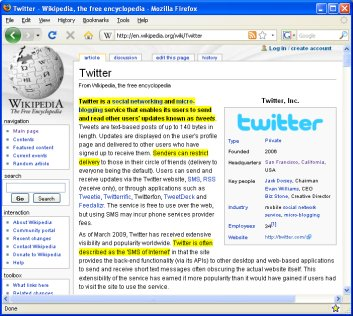
\includegraphics[width=2.5in]{figures/yawas}
  \caption{Annotation in Yawas}\label{fig:yawas}
\end{figure}

Feature-wise the system is much weaker than the previously analyzed brat (and much older),
however it contains a potentially useful idea: user-specific annotations which can later
be made accessible only to specific users or groups of users.

\subsection{Annotatie Systeem Annotation Tool} % Roman numerals
Annotatie~\cite{annotatie:on} is an annotation tool for printed
documents and belongs to the static annotation category.\vspace{10pt}

The anchoring of the annotations is done by page positioning: this seems inflexible at a
first glance, however, it constitutes a good alternative when the text in the page is not
digitized.  The feature that caught our attention is the extensive comment sectioned
derived from the annotations:
\begin{itemize}
\item Each annotation represents a new comment thread.
\item In each comment thread other users can further discuss on both the contents of the
  annotated text and the annotation itself.
\item All the annotations in a page are displayed in the right side of the page, as
  collapsed threads.
\end{itemize}
We believe that allowing discussion based on one user's annotation is an important feature
in such a system, as the context introduced by annotations is one which emphases user
collaboration.


%%% Local Variables: 
%%% mode: latex
%%% TeX-master: "kat"
%%% End: 
